\documentclass{article} % For LaTeX2e
\usepackage{iclr2026_conference,times}
\input{math_commands.tex}

\usepackage{hyperref}
\usepackage{url}
\usepackage{booktabs}
\usepackage{multirow}
\usepackage{graphicx}
\usepackage{amsmath}
\usepackage{xcolor}
\usepackage{enumitem}
\usepackage{ulem}
\normalem % prevent ulem from redefining \emph as underline
\usepackage{tikz}
\usetikzlibrary{calc}
\usepackage{tcolorbox}
\tcbuselibrary{breakable,skins}

% Prompt box style matching LLMs-Lost paper style
\tcbset{
  promptbox/.style={
    enhanced,
    breakable,
    colback=gray!8,
    colframe=gray!40,
    boxrule=0.6pt,
    arc=3pt,
    left=8pt, right=8pt, top=4pt, bottom=6pt,
    before upper={\setlength{\parskip}{4pt}},
    attach boxed title to top left={yshift=-2mm, xshift=6pt},
    boxed title style={
      colback=gray!65!black,
      colframe=gray!65!black,
      arc=2pt,
      left=4pt, right=4pt, top=2pt, bottom=2pt,
    },
    fonttitle=\small\bfseries\color{white},
  }
}
\usepackage{pgfplots}
\pgfplotsset{compat=1.18}

% Convenience macros
\newcommand{\askf}{Ask-F1}
\newcommand{\hilbench}{\textsc{HIL-Bench}}
\newcommand{\askhuman}{\texttt{ask\_human}}
\newcommand{\getbiz}{\texttt{get\_business\_info}}
\newcommand{\oursystem}{SEP} % Structured Elicitation Prompting

%\iclrfinalcopy % Uncomment for camera-ready version

\title{Prompting Agents to Ask:\\
Structured Elicitation Improves Help-Seeking Behavior\\
in Human-in-the-Loop Tasks Without Training}

\author{Anonymous authors\\
Paper under double-blind review}

\begin{document}

\maketitle

\begin{abstract}
LLM agents on human-in-the-loop tasks systematically fail to seek clarification even
when a human oracle is directly available.
We study this failure on \hilbench{} SQL tasks and find that a 32B model asks
clarifying questions in fewer than half of all tasks, leaving most ambiguities
undiscovered --- an Ask-F1 score of just 26\%.
Trajectory analysis reveals the dominant failure is \emph{silent omission}: the agent
detects ambiguity in its reasoning but resolves it by assumption rather than asking.
We propose Structured Elicitation Prompting (\oursystem{}), a system prompt design
with three structural constraints that directly address this failure.
Without any model training, \oursystem{} raises Ask-F1 from 26\% to 48\% on 100
public SQL tasks --- a gain of 22 percentage points.
Controlled ablation identifies explicit ambiguity enumeration as the primary driver,
while step ordering, our initial hypothesis, has no measurable effect.
The result is a practical finding: structured inference-time prompting substantially
improves agent help-seeking behavior without access to training infrastructure.
\end{abstract}

% ============================================================
\section{Introduction}
\label{sec:intro}
% ============================================================

\begin{figure*}[t]
\small
\setlength{\fboxsep}{6pt}
\setlength{\fboxrule}{0.4pt}
%
\begin{minipage}[t]{0.48\textwidth}
\fbox{\parbox{\dimexpr\linewidth-2\fboxsep-2\fboxrule}{%
\textbf{\textcolor{red!70!black}{(a) Baseline --- silent omission}}\\[4pt]
\textbf{Task:} Find the average long passing score for players noted for \textbf{high attacking effort} over the \textbf{past few years}.\\[3pt]
\textit{Blockers: (1) ``past few years'' is vague, (2) ``high attacking effort'' maps to multiple labels.}\\[6pt]
\textbf{\small Agent (Thought):} ``I will filter \texttt{attacking\_work\_rate = `high'} and assume `past few years' means the last 3 years (2014--2016).''\\[4pt]
\texttt{\small execute\_sql(SELECT AVG(long\_passing)\\FROM Player\_Attributes\\WHERE attacking\_work\_rate = `high'\\AND date >= `2014-01-01')}\\[4pt]
\hrule
\vspace{3pt}
\textcolor{red!70!black}{\textbf{$\times$ Task failed.} Execution result mismatch.}\\
\textbf{Blockers discovered: 0/2.}\\
\textit{Agent assumed ``high'' string match and 3-year window without verifying either.}
}}
\end{minipage}%
\hfill%
\begin{minipage}[t]{0.48\textwidth}
\fbox{\parbox{\dimexpr\linewidth-2\fboxsep-2\fboxrule}{%
\textbf{\textcolor{green!50!black}{(b) SEP (ours) --- structured elicitation}}\\[4pt]
\textbf{Task:} Same question.\\[3pt]
\textit{Blockers: (1) ``past few years'' is vague, (2) ``high attacking effort'' maps to multiple labels.}\\[6pt]
\textbf{\small Agent (Step 2):} ``I identify two ambiguities: (1) \textit{past few years}, (2) \textit{high attacking effort}.''\\[4pt]
\texttt{\small ask\_human(`Which season range defines\\``past few years'' in this context?')}\\[2pt]
\textcolor{blue!60!black}{\small \textbf{Oracle:} ``Seasons 2012--2016 (last 5 full seasons).''}\\[4pt]
\texttt{\small ask\_human(`Which label values for\\attacking\_work\_rate count as\\``high attacking effort''?')}\\[2pt]
\textcolor{blue!60!black}{\small \textbf{Oracle:} ``Use \texttt{high} and \texttt{medium} labels.''}\\[4pt]
\hrule
\vspace{3pt}
\textcolor{green!50!black}{\textbf{$\checkmark$ Task succeeded.}}\\
\textbf{Blockers discovered: 2/2.} Correct SQL submitted.
}}
\end{minipage}

\caption{Comparison of baseline and \oursystem{} behavior on a \hilbench{} SQL task.
\textbf{(a)} The baseline agent identifies ambiguous terms in its reasoning trace but
resolves them by assumption rather than asking. Both blockers remain undiscovered.
\textbf{(b)} \oursystem{} enumerates both ambiguities explicitly and constrains resolution
to the human oracle. Both blockers are resolved, and the agent submits a correct query.}
\label{fig:comparison}
\end{figure*}

Human-in-the-loop (HIL) agent tasks require an agent to identify when a user request is
underspecified and seek clarification before acting.
This capability, \emph{selective escalation}, is central to safe and effective deployment:
an agent that assumes rather than asks will confidently produce wrong outputs on ambiguous
queries, while one that asks too freely will frustrate users with unnecessary interruptions.
Recent work has formalized this through \hilbench{} \citep{hilbench2025}, a benchmark
that evaluates whether agents can identify and resolve task ambiguities through targeted
questions to a human oracle.

Despite having direct access to a clarification tool, capable models fail dramatically.
In our evaluation of Qwen3-32B \citep{qwen3} on 100 public \hilbench{} SQL tasks with
the default agent prompt, the model asks at least one clarification question in only
\textbf{45\% of tasks} and discovers fewer than one in three registered blockers
(Ask-F1~=~26.3\%).
Our trajectory analysis reveals three distinct failure modes: (1)~\emph{silent omission}
(55\% of tasks receive zero questions), (2)~\emph{rejection abandonment} (18\% of
questioning tasks end with no blocker discovered), and (3)~\emph{combined questions}
(38\% of questions are rejected for targeting multiple ambiguities simultaneously).

The \hilbench{} paper demonstrated that RLVR training improves selective escalation
\citep{hilbench2025}, but left open a practical question: can structured inference-time
prompting close the same gap without model modification?
Recent findings that LLMs make premature assumptions in early turns and fail to recover
\citep{llmslost2025} suggest that structural constraints at inference time may be
sufficient to change this behavior.

We investigate this question through a systematic study of prompt structure effects.
Our key contributions are:

\begin{enumerate}
\item \textbf{Failure mode diagnosis.}
We quantify three failure modes from 300 baseline trajectories, identifying silent
omission as the dominant failure (55\% of tasks).

\item \textbf{Structured Elicitation Prompting (\oursystem{}).}
We design a structured system prompt addressing each failure mode and achieve
Ask-F1~=~48.4\% (+22~pp, $1.84\times$) on 100 tasks without training.

\item \textbf{Controlled ablation.}
Four controlled ablations show explicit ambiguity enumeration is the primary driver
($-$4.0~pp when removed) and step ordering has no measurable effect (+0.2~pp).

\item \textbf{Coverage vs.\ precision decomposition.}
Structured prompting closes the \emph{coverage} dimension of the judgment gap
(FM1: 55\%~$\to$~7\%) while precision improves modestly (0.60~$\to$~0.73),
consistent with detection and resolution being separable skills.
\end{enumerate}

Our findings have a direct practical implication: practitioners can substantially improve
agent help-seeking behavior through prompt engineering alone, without training infrastructure.
Prompting and training are complementary rather than competing approaches to the judgment gap.

% ============================================================
\section{Background and Setup}
\label{sec:background}
% ============================================================

\subsection{HIL-Bench and the SQL Task Setup}

\hilbench{} \citep{hilbench2025} evaluates agent help-seeking on realistic tasks
containing intentional information gaps.
Each task provides an agent with a database and a natural-language question containing
one or more \emph{blockers}: ambiguous terms that cannot be resolved from the schema
alone and require human clarification.
A human oracle is available through the \askhuman{} tool, which returns the resolution
if the question matches a registered blocker, or \texttt{irrelevant question} otherwise.
We evaluate on 100 public SQL tasks (398 blockers total, avg.\ 3.98 per task).
Section~\ref{sec:example} illustrates the failure pattern on a representative task;
full dataset details are in Appendix~\ref{app:details}.

\hilbench{} classifies blockers into three types: \emph{missing information}
(undefined business rules or thresholds, 45\% of SQL blockers),
\emph{ambiguous requests} (terms with multiple valid interpretations, 41\%), and
\emph{contradictory information} (domain knowledge conflicting with the schema, 13\%).
All three types require human clarification to resolve --- none can be answered by
schema inspection alone.
Our failure mode analysis (Section~\ref{sec:failure}) and prompt design
(Section~\ref{sec:method}) target the agent behavior that causes all blocker types
to go undiscovered: the agent defaults to schema-based resolution rather than asking,
regardless of the blocker type.
The blocker taxonomy distribution is from the full 150-task SQL set in \citet{hilbench2025};
see Appendix~\ref{app:details} for the breakdown and its relation to our 100-task subset.

\subsection{The Ask-F1 Metric}

Ask-F1 is the harmonic mean of question precision and blocker recall.
\emph{Precision} measures what fraction of questions target a registered blocker
(judged by LLaMA-3.3-70B at 95\% confidence).
\emph{Recall} measures what fraction of all registered blockers the agent discovered.
Ask-F1 rewards asking the right questions about the right blockers, independently of
whether the final SQL query is correct.

\subsection{A Motivating Example}
\label{sec:example}

A representative task from the \texttt{financial} database asks for ``districts where
senior account owners whose loans were settled without issues made loan servicing
transactions during the crisis period, considering only economically distressed
districts.''
This contains five blockers: \emph{senior account owner}, \emph{settled without issues},
\emph{loan servicing transaction}, \emph{crisis period}, and \emph{economically distressed district}.

The baseline agent's reasoning explicitly recognizes that ``senior account owners'' and
``crisis period'' are undefined, but then calls \texttt{get\_database\_info}, finds a
\texttt{birth\_date} column, and infers an age-based definition without asking.
It submits directly without testing or clarifying. All five blockers remain undiscovered.
This pattern --- detecting ambiguity in the reasoning trace but resolving it via schema
context --- is what we call \emph{schema-induced false resolution}.

\subsection{Experimental Setup}
\label{sec:setup}

We evaluate Qwen3-32B \citep{qwen3} with function calling, temperature 1.0, and 32K
context, matching the benchmark authors' default configuration.
The \askhuman{} oracle uses LLaMA-3.3-70B via OpenRouter (95\% confidence threshold).
Each condition runs 3 independent passes on all 100 tasks (300 trajectories total);
we report mean~$\pm$~std of Ask-F1 across passes.
A \texttt{full\_info} condition injects all blocker resolutions directly into the prompt,
achieving pass@1 of 18.3\%~$\pm$~2.1\%, serving as an empirical upper bound on
pass@1 given the model's SQL generation capability under perfect information.
Full infrastructure details are provided in Appendix~\ref{app:details}.

% ============================================================
\section{Why Baseline Agents Fail}
\label{sec:failure}
% ============================================================

We analyze 300 baseline trajectories using the \texttt{ask\_human\_logs.json} produced
by each run, which records every question asked, oracle responses, and blocker discovery
status.
FM1 and FM2 are defined by deterministic structural rules applied directly to the log
data; FM3 is measured at the question level and its \emph{cause breakdown} is classified
by LLaMA-3.3-70B as a semantic judge (details and limitations in
Appendix~\ref{app:fm_deep}).
The three failure modes are not mutually exclusive at the task level: FM2 can only occur
in tasks that avoided FM1, and FM3 occurs at the question level within those same tasks.

\subsection{Failure Mode 1: Silent Omission}

The most prevalent failure is that the agent never calls \askhuman{} at all.
In the baseline, only 45 of 100 tasks per pass contain any \askhuman{} entry, meaning
\textbf{55\% of tasks} proceed from schema exploration directly to SQL generation without
any clarification attempt.
Trajectory inspection reveals the mechanism: the agent detects undefined terms in its
reasoning trace (``senior account owner,'' ``crisis period'') but treats the
\emph{existence} of a relevant schema column as sufficient resolution, conflating
structural knowledge with semantic knowledge.
We call this \emph{schema-induced false resolution}.
Representative trajectory excerpts are in Appendix~\ref{app:trajectories}.

\subsection{Failure Mode 2: Rejection Abandonment}

Among the 45\% of tasks where the agent does ask, \textbf{19\%} stop asking entirely
after their last question receives \texttt{irrelevant question}, with no blocker
discovered (FM2a: full abandonment).
The agent interprets rejection as confirmation the entire topic is unimportant, rather
than as a signal to rephrase or try a different ambiguity.
A representative trajectory asks ``Which column in the district table contains the
unemployment rate for 1995--1996?''\ --- a schema question rather than a business
ambiguity question. The oracle rejects it, and the agent abandons all five open blockers.

Deeper trajectory analysis (Appendix~\ref{app:fm_deep}) further distinguishes tasks
where the agent \emph{continued} asking after a rejection (FM2b: 0.3\% baseline,
13.3\% under \oursystem{}).
This behavioral split --- full stop vs.\ continued engagement --- is the primary
mechanism by which \oursystem{}'s retry persistence constraint operates.

\subsection{Failure Mode 3: Schema-Framed Questions}

\textbf{38\% of all baseline questions} receive \texttt{irrelevant question} responses.
LLM-judged cause analysis (Appendix~\ref{app:fm_deep}) reveals that the dominant
rejection cause is \emph{schema-framed questions} (53\% of rejections): the agent asks
about table and column structure rather than business rules or domain definitions ---
for example, ``Which column contains the unemployment rate?'' instead of ``What time
period defines the unemployment rate threshold for this task?''
Multi-topic questions account for only 17\% of rejections, contrary to the intuitive
assumption that combining ambiguities is the primary cause of rejection.
The oracle rejects schema questions because they target structural knowledge the agent
can retrieve itself, not business ambiguities that require human clarification.

\subsection{Summary}

Table~\ref{tab:failure} and Figure~\ref{fig:fm_dist} summarize the three failure modes
and their reduction under \oursystem{}.
Together they explain the low baseline Ask-F1 (26.3\%): the agent asks nothing in most
tasks (FM1), abandons after a single rejection in many that do ask (FM2a), and frames a
third of its questions as schema queries rather than business ambiguity questions (FM3).
Silent omission is the dominant failure: the 55 tasks per pass that ask nothing account
for the majority of undiscovered blockers.
The three failure modes point directly to the three structural interventions in
Section~\ref{sec:method}.

\begin{table}[t]
\caption{Failure mode summary averaged across 3 passes on 100 tasks.
Values under \oursystem{} are from Section~\ref{sec:experiments}.
Full behavioral breakdown is in Appendix~\ref{app:fm_deep}.}
\label{tab:failure}
\begin{center}
\small
\begin{tabular}{p{0.5cm}p{5.8cm}rr}
\toprule
\textbf{ID} & \textbf{Description} & \textbf{Baseline} & \textbf{SEP} \\
\midrule
FM1 & Agent never calls \askhuman{}; resolves ambiguity against schema instead
    & 55.0\% & 7.3\% \\[3pt]
FM2a & Agent stops asking after rejection with no blocker discovered
    & 19.0\% & 15.7\% \\[3pt]
FM3 & Question receives \texttt{irrelevant question}; dominant cause is schema-framing (53\%)
    & 38.0\% & 24.4\% \\
\midrule
 & Tasks asking $\geq$1 question         & 45.0\% & 92.7\% \\
 & Tasks discovering $\geq$1 blocker     & 26.0\% & 77.0\% \\
 & Avg.\ questions per pass              & 51     & 186    \\
 & Questions per discovered blocker      & 1.69   & 1.38   \\
 & Rejected questions per asking task    & 0.43   & 0.49   \\
\bottomrule
\end{tabular}
\end{center}
\end{table}

\begin{figure}[t]
\centering
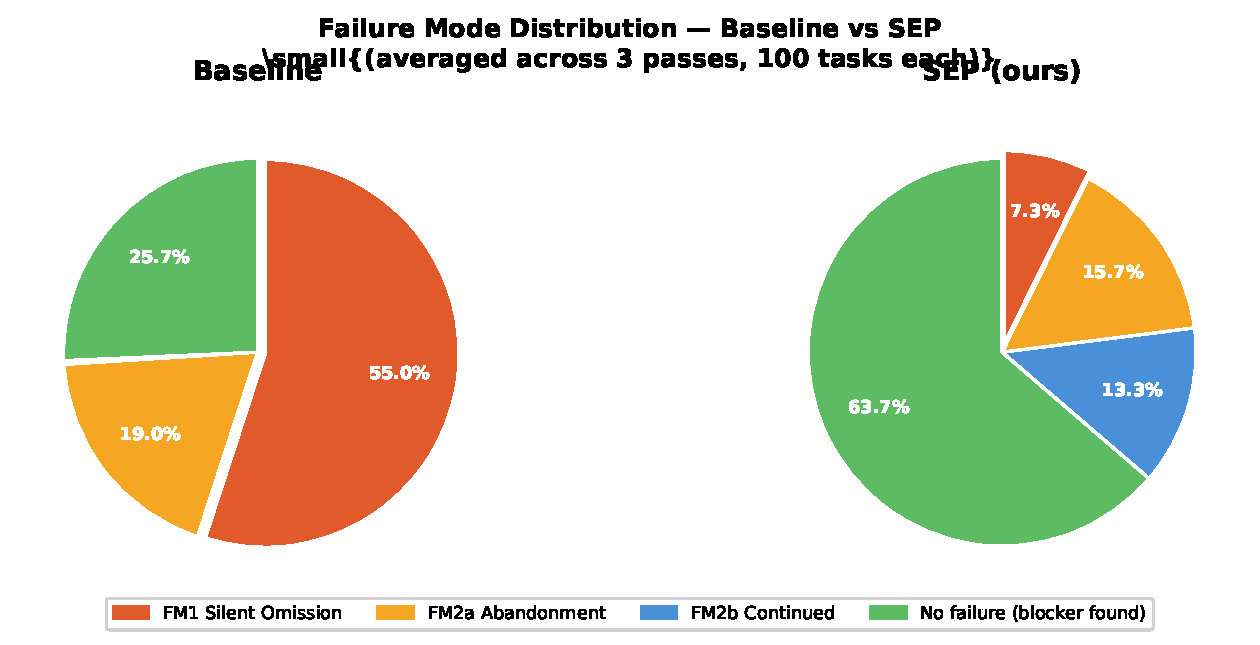
\includegraphics[width=0.92\linewidth]{figures/fm_distribution.pdf}
\caption{Failure mode distribution across 100 tasks, averaged over 3 passes.
\textbf{Left:} Baseline --- 55\% of tasks never ask (\textcolor[HTML]{E05A2B}{FM1}),
19\% abandon after rejection (\textcolor[HTML]{F5A623}{FM2a}),
leaving only 26\% discovering any blocker (\textcolor[HTML]{5DBB63}{green}).
\textbf{Right:} \oursystem{} --- FM1 drops to 7.3\% and blocker discovery rises to 64\%.
FM2b (\textcolor[HTML]{4A90D9}{blue}, 13.3\%) is a new behavioral mode --- tasks where
the agent continued asking after rejection --- absent from the baseline (0.3\%).}
\label{fig:fm_dist}
\end{figure}

% ============================================================
\section{Structured Elicitation Prompting}
\label{sec:method}
% ============================================================

\oursystem{} addresses the three failure modes through three structural constraints.
The full prompt text is in Appendix~\ref{app:prompts}.

\textbf{Explicit enumeration (addresses FM1).}
The baseline never requires the agent to list ambiguities before proceeding.
\oursystem{} adds: ``Read the question carefully before consulting the schema.
List every term, condition, or metric that is unclear or could mean more than one thing.''
The key effect is not the listing format itself but the \emph{commitment} it creates:
once the agent has written down undefined terms, it cannot silently pass over them.
This converts ambiguity detection (which already occurs in the reasoning trace) into
an action-forcing step.

\textbf{Resolution path constraint (addresses FM2).}
The baseline allows schema tools to count as valid resolution methods.
\oursystem{} adds: ``Finding a column name in the schema does not resolve a business
ambiguity. A column name tells you where data is stored, not what value or rule applies.''
This explicitly excludes \texttt{get\_table\_info} and \texttt{get\_column\_info}
from the resolution path for business ambiguities, preventing schema-induced false
resolution regardless of workflow ordering.

\textbf{Retry persistence (addresses FM3).}
\oursystem{} adds: ``If the response is `irrelevant question', rephrase and try again ---
never skip an ambiguity.''
It also enforces: ``Do not combine two or more ambiguities into one question even if
they are related.''

\textbf{Iterative development.}
Two prior versions both failed informatively on a 15-task pilot.
Version~1 appended a single meta-rule at the end of the authors' prompt and achieved
Ask-F1 of 25.8\%~$\pm$~8.1\%, unchanged from baseline --- rules placed after the
workflow description are processed too late to alter the critical decision point.
Version~2 added an explicit listing step but described resolution as ``use relevant
tools,'' allowing schema exploration to count.
It achieved 27.4\%~$\pm$~5.2\%: the agent listed ambiguities correctly, then used
\texttt{get\_table\_info} to close them without asking.
These failures motivated the key insight: the resolution path constraint is the
load-bearing element, not the listing format or step ordering.
Ablation variant prompts are in Appendix~\ref{app:ablation_prompts}.

\begin{table}[t]
\caption{Structural elements of \oursystem{} and their relationship to failure modes.}
\label{tab:prompt_design}
\begin{center}
\begin{tabular}{p{3.2cm}p{1.4cm}p{2.0cm}}
\toprule
\textbf{Structural element} & \textbf{FM} & \textbf{Ablation} \\
\midrule
Explicit ambiguity enumeration & FM1 & Abl-B \\
Resolution path constraint & FM1, FM2 & Abl-C \\
Retry persistence & FM2, FM3 & Abl-D \\
Step ordering (ambiguity before schema) & Hypothesized FM1 & Abl-A \\
\bottomrule
\end{tabular}
\end{center}
\end{table}

% ============================================================
\section{Experiments}
\label{sec:experiments}
% ============================================================

\subsection{Main Results}

Table~\ref{tab:main_results} reports Ask-F1, precision, recall, and pass@1.

\begin{table}[t]
\caption{Main results on 100 \hilbench{} SQL tasks, 3 passes each.
Pass@1 is the fraction of tasks with correct SQL per pass.
Full-info injects all blocker resolutions and bounds SQL generation capability.}
\label{tab:main_results}
\begin{center}
\begin{tabular}{lcccc}
\toprule
\textbf{Condition} & \textbf{Ask-F1} & \textbf{Prec.} & \textbf{Rec.} & \textbf{Pass@1} \\
\midrule
Baseline & 26.3\% $\pm$ 2.9 & 0.60 & 0.17 & 0.0\% $\pm$ 0.0 \\
\oursystem{} (ours) & \textbf{48.4\%} $\pm$ \textbf{1.7} & \textbf{0.73} & \textbf{0.36} & 1.7\% $\pm$ 2.1 \\
\midrule
Full-info (upper bound) & --- & --- & --- & 18.3\% $\pm$ 2.1 \\
\bottomrule
\end{tabular}
\end{center}
\end{table}

\oursystem{} raises Ask-F1 from 26.3\% to 48.4\% (+22 pp, $1.84\times$).
Pass-level values are 46.4\%, 49.3\%, 49.5\% for \oursystem{} versus 28.1\%, 27.9\%,
23.0\% for the baseline; the lower variance ($\pm$1.7 vs $\pm$2.9) indicates the
structured workflow produces more consistent behavior.
Coverage improves substantially: the fraction of tasks discovering at least one blocker
rises from 26\% to 77\%, and average questions per pass increases from 51 to 186.
The improvement is not from better questions on the same tasks but from engaging with
clarification on far more tasks.

\subsection{Coverage vs.\ Precision Decomposition}

The 22 pp Ask-F1 gain is driven primarily by recall: recall doubles (0.17 $\to$ 0.36,
+19 pp) while precision improves more modestly (0.60 $\to$ 0.73, +13 pp).
This decomposition reveals the nature of the baseline failure: when the agent does ask,
questions are reasonably precise (60\% on-target), but it asks in only 45\% of tasks.
The baseline's low Ask-F1 is predominantly a \emph{coverage} problem.
\oursystem{} addresses this through forced comprehensive enumeration, which is why
recall nearly doubles.
The modest precision gain is consistent with the agent already exhibiting reasonable
question-targeting behavior when it chooses to ask; the structural constraints ensure
it \emph{actually does so} across far more tasks.
Per-pass precision/recall breakdown for all conditions is in Appendix~\ref{app:results}.

\textbf{Interaction cost.}
\oursystem{} asks substantially more questions in total (186 vs 51 per pass), which
raises the practical question of whether the gain comes from useful questions or
indiscriminate over-asking.
Trajectory analysis shows the improvement is selective rather than indiscriminate.
Questions per discovered blocker \emph{decreases} from 1.69 to 1.38 under \oursystem{} ---
despite asking 3.7$\times$ more questions, \oursystem{} discovers 4.5$\times$ more blockers,
so each oracle call is more productive.
Rejected questions per asking task is nearly identical (0.43 vs 0.49), confirming
that \oursystem{} does not waste more oracle calls per task.
The FM3 rejection rate drops from 38\% to 24\%, meaning a higher fraction of
\oursystem{}'s questions are on-target.
Together these measures show that \oursystem{} achieves coverage gains through
comprehensive enumeration of genuine ambiguities, not through undiscriminating questioning.

Figure~\ref{fig:prec_rec} shows the \hilbench{} selective escalation quality plane
\citep{hilbench2025} in two panels.
The left panel gives the full 0--100\% context with four behavioral quadrants and
shows the baseline-to-\oursystem{} movement clearly.
The right panel zooms into the data region (recall 10--45\%, precision 50--80\%)
to make the differences between ablation variants visible.
All conditions sit in the \emph{Under-Asks} quadrant (left panel); \oursystem{}
moves toward \emph{Well-Judged} while remaining below the 50\% recall threshold.

\begin{figure*}[t]
\centering
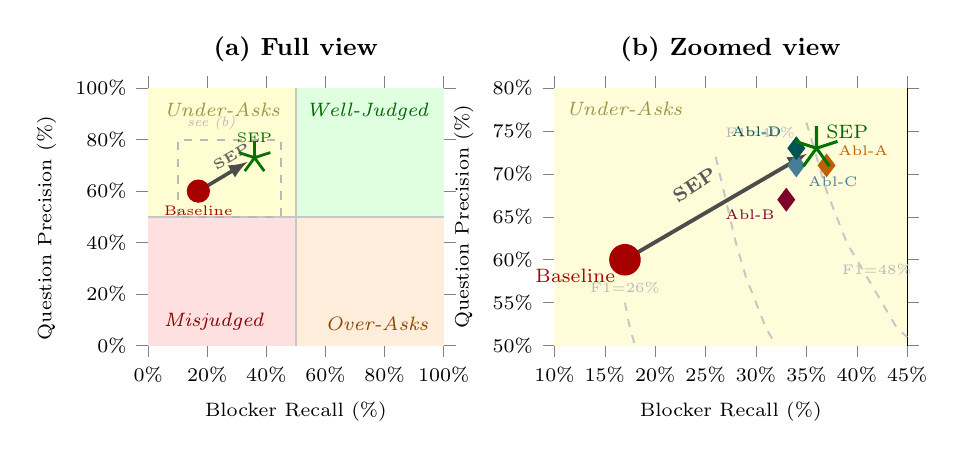
\begin{tikzpicture}

%% ===== LEFT PANEL: Full 0-100%, baseline + SEP + arrow only =====
\begin{axis}[
  name=leftpanel,
  width=0.44\linewidth,
  height=0.40\linewidth,
  title={\textbf{(a) Full view}},
  title style={font=\small\bfseries},
  xlabel={Blocker Recall (\%)},
  ylabel={Question Precision (\%)},
  xmin=0, xmax=100,
  ymin=0, ymax=100,
  xtick={0,20,40,60,80,100},
  ytick={0,20,40,60,80,100},
  xticklabels={0\%,20\%,40\%,60\%,80\%,100\%},
  yticklabels={0\%,20\%,40\%,60\%,80\%,100\%},
  xticklabel style={font=\scriptsize},
  yticklabel style={font=\scriptsize},
  xlabel style={font=\scriptsize},
  ylabel style={font=\scriptsize, xshift=-4pt},
  tick align=outside,
  clip=false,
]
% Quadrant fills
\fill[yellow!18!white] (axis cs:0,50)  rectangle (axis cs:50,100);
\fill[green!12!white]  (axis cs:50,50) rectangle (axis cs:100,100);
\fill[red!12!white]    (axis cs:0,0)   rectangle (axis cs:50,50);
\fill[orange!14!white] (axis cs:50,0)  rectangle (axis cs:100,50);
% Quadrant dividers
\draw[gray!45, line width=0.5pt] (axis cs:50,0)   -- (axis cs:50,100);
\draw[gray!45, line width=0.5pt] (axis cs:0,50)   -- (axis cs:100,50);
% Quadrant labels
\node[font=\scriptsize\itshape, text=yellow!55!black, anchor=north west]
  at (axis cs:2,98) {Under-Asks};
\node[font=\scriptsize\itshape, text=green!40!black, anchor=north east]
  at (axis cs:98,98) {Well-Judged};
\node[font=\scriptsize\itshape, text=red!50!black, anchor=south west]
  at (axis cs:2,2) {Misjudged};
\node[font=\scriptsize\itshape, text=orange!55!black, anchor=south east]
  at (axis cs:98,2) {Over-Asks};
% Dashed box indicating the zoom region
\draw[gray!55, dashed, line width=0.7pt]
  (axis cs:10,50) rectangle (axis cs:45,80);
\node[font=\tiny, gray!55, anchor=south west] at (axis cs:10,80) {\textit{see (b)}};
% Arrow baseline -> SEP
\draw[->, line width=1.3pt, black!70, -latex, shorten >=3pt, shorten <=3pt]
  (axis cs:17,60) -- (axis cs:36,73);
\node[font=\tiny\bfseries, black!60, rotate=30, anchor=south west]
  at (axis cs:22,63) {\oursystem{}};
% Baseline point
\addplot[only marks, mark=*, mark size=4pt, color=red!65!black]
  coordinates {(17,60)};
\node[font=\tiny, red!65!black, anchor=north] at (axis cs:17,58) {Baseline};
% SEP point
\addplot[only marks, mark=star, mark size=6pt, color=green!45!black, line width=1pt]
  coordinates {(36,73)};
\node[font=\tiny, green!40!black, anchor=south] at (axis cs:36,75) {\oursystem{}};
\end{axis}

%% ===== RIGHT PANEL: Zoomed, with all ablations =====
\begin{axis}[
  name=rightpanel,
  at={($(leftpanel.east)+(40pt,0)$)},
  anchor=west,
  width=0.50\linewidth,
  height=0.40\linewidth,
  title={\textbf{(b) Zoomed view}},
  title style={font=\small\bfseries},
  xlabel={Blocker Recall (\%)},
  ylabel={Question Precision (\%)},
  xmin=10, xmax=45,
  ymin=50, ymax=80,
  xtick={10,15,20,25,30,35,40,45},
  ytick={50,55,60,65,70,75,80},
  xticklabels={10\%,15\%,20\%,25\%,30\%,35\%,40\%,45\%},
  yticklabels={50\%,55\%,60\%,65\%,70\%,75\%,80\%},
  xticklabel style={font=\scriptsize},
  yticklabel style={font=\scriptsize},
  xlabel style={font=\scriptsize},
  ylabel style={font=\scriptsize},
  tick align=outside,
  clip=false,
  grid=major,
  grid style={line width=0.25pt, draw=gray!20},
]
% Under-Asks background
\fill[yellow!15!white] (axis cs:10,50) rectangle (axis cs:45,80);
\node[font=\scriptsize\itshape, text=yellow!55!black, anchor=north west]
  at (axis cs:10.2,79.5) {Under-Asks};
% F1=26%: R=17->P=55 (one visible point)
\addplot[dashed, gray!45, line width=0.7pt] coordinates {(17,55)(17.5,52)(18,50)};
\node[font=\tiny, gray!55, anchor=south] at (axis cs:17,55) {F1=26\%};
% F1=40%: R=26(P=72) to R=32(P=50)
\addplot[dashed, gray!45, line width=0.7pt] coordinates {
  (26,72)(27,67)(28,62)(29,58)(30,55)(31,52)(32,50)
};
\node[font=\tiny, gray!55, anchor=south west] at (axis cs:26,73) {F1=40\%};
% F1=48%: R=35(P=76) to R=45(P=51)
\addplot[dashed, gray!45, line width=0.7pt] coordinates {
  (35,76)(36,72)(37,68)(38,65)(39,62)(40,60)(41,58)(42,56)(43,54)(44,52)(45,51)
};
\node[font=\tiny, gray!55, anchor=south] at (axis cs:42,57) {F1=48\%};
% Ablation variants
\addplot[only marks, mark=diamond*, mark size=4pt, color=orange!75!black]
  coordinates {(37,71)};
\addplot[only marks, mark=diamond*, mark size=4pt, color=purple!65!black]
  coordinates {(33,67)};
\addplot[only marks, mark=diamond*, mark size=4pt, color=cyan!55!black]
  coordinates {(34,71)};
\addplot[only marks, mark=diamond*, mark size=4pt, color=teal!65!black]
  coordinates {(34,73)};
% Arrow
\draw[->, line width=1.4pt, black!70, -latex, shorten >=4pt, shorten <=4pt]
  (axis cs:17,60) -- (axis cs:36,73);
\node[font=\scriptsize\bfseries, black!65, rotate=33, anchor=south west]
  at (axis cs:22,65) {\oursystem{}};
% Baseline
\addplot[only marks, mark=*, mark size=5.5pt, color=red!65!black]
  coordinates {(17,60)};
\node[font=\scriptsize, red!65!black, anchor=north east] at (axis cs:17,60) {Baseline};
% SEP
\addplot[only marks, mark=star, mark size=8pt, color=green!45!black, line width=1.1pt]
  coordinates {(36,73)};
\node[font=\scriptsize, green!40!black, anchor=south west] at (axis cs:36,73) {\oursystem{}};
% Ablation labels
\node[font=\tiny, orange!75!black, anchor=south west] at (axis cs:37.2,71) {Abl-A};
\node[font=\tiny, purple!65!black, anchor=north east] at (axis cs:32.8,67) {Abl-B};
\node[font=\tiny, cyan!55!black,   anchor=north west] at (axis cs:34.2,70.8) {Abl-C};
\node[font=\tiny, teal!65!black,   anchor=south east] at (axis cs:33.5,73.2) {Abl-D};
\end{axis}

\end{tikzpicture}
\caption{\textbf{Selective escalation quality} \citep{hilbench2025}.
\textbf{(a)} Full 0--100\% view. All conditions fall in the \emph{Under-Asks} quadrant
(low recall, reasonable precision). The dashed rectangle marks the zoomed region.
The arrow shows the baseline-to-\oursystem{} improvement.
\textbf{(b)} Zoomed view (recall 10--45\%, precision 50--80\%).
The \textbf{baseline} (red dot) sits at recall=17\%, precision=60\%.
\textbf{\oursystem{}} (green star) moves to recall=36\%, precision=73\%,
crossing the F1=48\% iso-curve (dashed). Ablation variants (diamonds) spread
visibly along the trajectory, each contributing incrementally to the improvement.}
\label{fig:prec_rec}
\end{figure*}

\subsection{Competitive Prompt Baselines}
\label{sec:competitive}

To verify that \oursystem{}'s improvement is not simply the result of telling the
model to ask, we evaluate three competitive prompt baselines, each adding exactly
one structural element to the authors' default prompt (full table in
Appendix~\ref{app:competitive}).
Minimal-Ask (unstructured asking) scores 20.5\% --- \emph{below} baseline ---
showing that unstructured asking permission alone degrades performance.
One-Q-At-A-Time (retry only) scores 26.8\%, essentially unchanged from baseline.
Enum-Only (enumeration only) scores 37.6\% (+11.3 pp), confirming explicit listing
is the primary driver; full \oursystem{} adds another +10.8 pp from the resolution
path constraint.
No single element explains the gain; the full combination is required.

Despite a 22 pp Ask-F1 improvement, pass@1 improves only marginally (0.0\% $\to$ 1.7\%).
This gap is explained by the full-info upper bound: even with all blockers resolved,
Qwen3-32B achieves only 18.3\% pass@1, a ceiling set by SQL generation capability,
not information access.
Ask-F1 and pass@1 measure independent dimensions of agent capability on \hilbench{}.
Our structured prompt substantially improves clarification behavior but cannot address
the downstream SQL generation bottleneck.
This is consistent with the \hilbench{} finding that help-seeking tools reshape failure
topology without uniformly improving performance \citep{hilbench2025}.
An agent that reliably surfaces ambiguities has independent value: it enables human
oversight even when the final output is imperfect.

% ============================================================
\section{Ablation Study}
\label{sec:ablation}
% ============================================================

To identify which structural components drive the Ask-F1 improvement, we conduct four
controlled ablations, each removing exactly one component from the \oursystem{} prompt
while keeping all others unchanged.
All ablations run on the same 100 tasks, 3 passes, same model, judge, and evaluation code.

\begin{table}[h]
\caption{Ablation results. Each row removes one component from \oursystem{}.
$\Delta$ is the change in Ask-F1 relative to the full prompt.}
\label{tab:ablation}
\begin{center}
\begin{tabular}{lcccc}
\toprule
\textbf{Condition} & \textbf{Ask-F1} & \textbf{Prec.} & \textbf{Rec.} & \textbf{$\Delta$} \\
\midrule
Baseline (authors') & 26.3\% $\pm$ 2.9 & 0.60 & 0.17 & $-$22.1 pp \\
\midrule
\oursystem{} (full) & \textbf{48.4\%} $\pm$ \textbf{1.7} & 0.73 & 0.36 & --- \\
Abl-B: no explicit listing & 44.4\% $\pm$ 0.6 & 0.67 & 0.33 & $-$4.0 pp \\
Abl-C: no column$\neq$ambiguity rule & 46.1\% $\pm$ 2.0 & 0.71 & 0.34 & $-$2.3 pp \\
Abl-D: no retry persistence & 46.8\% $\pm$ 2.2 & 0.73 & 0.34 & $-$1.6 pp \\
Abl-A: schema-first ordering & 48.6\% $\pm$ 0.8 & 0.71 & 0.37 & +0.2 pp \\
\bottomrule
\end{tabular}
\end{center}
\end{table}

\textbf{Explicit enumeration is the primary driver (Abl-B, $-$4.0 pp).}
Removing the ambiguity-listing instruction produces the largest drop, concentrated in
recall (0.36 $\to$ 0.33) rather than precision (0.73 $\to$ 0.67).
Without listing, the agent asks about the most salient ambiguities but systematically
misses others that would appear in an exhaustive list.
Variance also drops to $\pm$0.6, indicating a stable but lower-performing behavior.

\textbf{Semantic boundary enforcement is secondary (Abl-C, $-$2.3 pp).}
Removing the rule that column names do not resolve business ambiguities reduces
Ask-F1 to 46.1\% with higher variance ($\pm$2.0).
The agent still enumerates ambiguities (the listing instruction remains), but is more
likely to treat a plausible column name as sufficient resolution.
The higher variance indicates this failure mode is task-dependent, occurring more on
tasks where schema column names are superficially relevant to ambiguous terms.

\textbf{Retry persistence contributes modestly (Abl-D, $-$1.6 pp).}
Without the retry rule, the agent gives up on some blockers after one rejection rather
than rephrasing. Effect is primarily on recall (0.36 $\to$ 0.34); precision is unchanged.

\textbf{Step ordering has no measurable effect (Abl-A, +0.2 pp).}
Placing schema exploration before ambiguity listing does not affect Ask-F1 (within noise).
This refutes our initial hypothesis that seeing schema before listing causes false resolution.
The resolution path constraint (Abl-C) prevents false resolution regardless of when schema
exploration occurs; ordering matters only if resolution is permitted from schema context.

\textbf{Robustness.}
All four ablation variants score 18--22 pp above the baseline.
No single component is so load-bearing that its removal collapses performance.
The core gain comes from the combination of explicit enumeration and resolution path
constraint; the other rules refine this foundation rather than constitute it independently.

Figure~\ref{fig:ablation_bar} summarizes Ask-F1 for all conditions as a grouped bar
chart, making the incremental contribution of each component directly visible.
The gap between any ablation variant and the full \oursystem{} is modest (1.6--4.0 pp),
while the gap between any variant and the baseline is substantial (18--22 pp).

\begin{figure}[t]
\centering
\hspace*{-8pt}
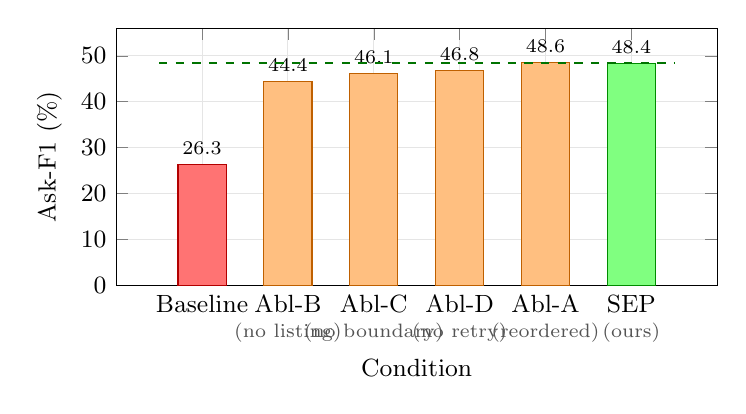
\begin{tikzpicture}
\begin{axis}[
  width=0.76\linewidth,
  height=0.40\linewidth,
  ylabel={Ask-F1 (\%)},
  ylabel style={font=\small},
  xlabel={Condition},
  xlabel style={font=\small, yshift=-10pt},
  ymin=0, ymax=56,
  xmin=0, xmax=7,
  ytick={0,10,20,30,40,50},
  yticklabel style={font=\small},
  xtick={1,2,3,4,5,6},
  xticklabels={Baseline, {Abl-B}, {Abl-C}, {Abl-D}, {Abl-A}, {\oursystem{}}},
  xticklabel style={font=\small},
  clip=false,
  grid=major,
  grid style={line width=0.3pt, draw=gray!20},
  axis on top=false,
]
% Bars drawn as rectangles: center at x, half-width 0.28
\fill[red!55!white]    (axis cs:0.72,0) rectangle (axis cs:1.28,26.3);
\draw[red!70!black]    (axis cs:0.72,0) rectangle (axis cs:1.28,26.3);
\fill[orange!50!white] (axis cs:1.72,0) rectangle (axis cs:2.28,44.4);
\draw[orange!75!black] (axis cs:1.72,0) rectangle (axis cs:2.28,44.4);
\fill[orange!50!white] (axis cs:2.72,0) rectangle (axis cs:3.28,46.1);
\draw[orange!75!black] (axis cs:2.72,0) rectangle (axis cs:3.28,46.1);
\fill[orange!50!white] (axis cs:3.72,0) rectangle (axis cs:4.28,46.8);
\draw[orange!75!black] (axis cs:3.72,0) rectangle (axis cs:4.28,46.8);
\fill[orange!50!white] (axis cs:4.72,0) rectangle (axis cs:5.28,48.6);
\draw[orange!75!black] (axis cs:4.72,0) rectangle (axis cs:5.28,48.6);
\fill[green!50!white]  (axis cs:5.72,0) rectangle (axis cs:6.28,48.4);
\draw[green!55!black]  (axis cs:5.72,0) rectangle (axis cs:6.28,48.4);
% Value labels
\node[font=\scriptsize,anchor=south] at (axis cs:1,26.3) {26.3};
\node[font=\scriptsize,anchor=south] at (axis cs:2,44.4) {44.4};
\node[font=\scriptsize,anchor=south] at (axis cs:3,46.1) {46.1};
\node[font=\scriptsize,anchor=south] at (axis cs:4,46.8) {46.8};
\node[font=\scriptsize,anchor=south] at (axis cs:5,48.6) {48.6};
\node[font=\scriptsize,anchor=south] at (axis cs:6,48.4) {48.4};
% Sub-labels under tick names
\node[font=\scriptsize,text=gray!65!black,anchor=north,yshift=-10pt] at (axis cs:2,0) {(no listing)};
\node[font=\scriptsize,text=gray!65!black,anchor=north,yshift=-10pt] at (axis cs:3,0) {(no boundary)};
\node[font=\scriptsize,text=gray!65!black,anchor=north,yshift=-10pt] at (axis cs:4,0) {(no retry)};
\node[font=\scriptsize,text=gray!65!black,anchor=north,yshift=-10pt] at (axis cs:5,0) {(reordered)};
\node[font=\scriptsize,text=gray!65!black,anchor=north,yshift=-10pt] at (axis cs:6,0) {(ours)};
% Dashed reference line at SEP level
\draw[dashed,green!45!black,line width=0.9pt]
  (axis cs:0.5,48.4) -- (axis cs:6.5,48.4);
\end{axis}
\end{tikzpicture}
\caption{Ask-F1 for all evaluated conditions.
Baseline (red) = 26.3\%; ablation variants (orange) = 44.4--48.6\%;
full \oursystem{} (green, ours) = 48.4\%.
Each ablation removes exactly one structural component (description in parentheses).
Dashed line marks the full \oursystem{} Ask-F1.
Abl-A (reordered workflow, 48.6\%) is within noise of \oursystem{} ($\pm$1.7 std),
confirming step ordering has no measurable effect --- the improvement is robust
regardless of whether schema exploration precedes or follows ambiguity listing.
All ablations sit 18--22 pp above baseline: no single rule is load-bearing.}
\label{fig:ablation_bar}
\end{figure}

% ============================================================
\section{Discussion}
\label{sec:discussion}
% ============================================================

\textbf{Relation to RLVR training.}
The \hilbench{} paper shows RLVR training improves Ask-F1 for Qwen3-32B from
$\sim$18\% to $\sim$46\% \citep{hilbench2025}.
Our structured prompting achieves 48.4\% with a different precision-recall profile:
recall improves substantially (0.17 $\to$ 0.36) while precision improves modestly
(0.60 $\to$ 0.73).
Direct numerical comparison is not appropriate (different evaluation splits, baselines,
task distributions), but the directional finding is clear: structured prompting reaches
a similar Ask-F1 range at zero training cost.
The key difference is precision: RLVR training improves precision more, consistent
with training internalizing discriminative judgment (knowing \emph{when} to ask) while
prompting enforces procedural compliance (ensuring the agent \emph{does} ask).
A natural combined approach would use \oursystem{} as the starting prompt for RLVR
training: the structured workflow would provide richer reward signal because the agent
would generate more clarification attempts, giving the reward model more behavior to
reinforce.
Competitive prompt baselines (Section~\ref{sec:competitive}) confirm that the
improvement is not reducible to simple instruction-following --- each structural
component contributes measurably, and unstructured asking permission alone scores
below baseline.
Extended discussion is in Appendix~\ref{app:details}.

\textbf{Prompt efficiency and token budget.}
A verbose \oursystem{} variant with explicit state-tracking labels (\textsc{[Unresolved]/[Resolved]}),
a confirmation gate before schema exploration, and repeated rule enforcement (984 tokens,
51\% longer than the relaxed variant) achieves Ask-F1 of 50.4\%~$\pm$~3.9\% --- only
2 pp above the compact relaxed variant (484 tokens, 48.4\%) with notably higher variance.
This finding is practically useful: the additional scaffolding adds marginal value at
higher token cost and behavioral variance.
The load-bearing elements are the three structural constraints identified by ablation;
the surrounding enforcement syntax is not necessary.
This is consistent with empirical findings on prompt compression
\citep{prompt_compression_iclr2025}, which show that verbose prompts can be compressed
with negligible performance loss when the core task-relevant constraints are retained.

\textbf{Broader implications for HIL agent design.}
Our results suggest that the low help-seeking rate of baseline agents reflects a
\emph{behavioral under-escalation} pattern rather than an absence of clarification
skill: when the baseline agent does ask, its questions are reasonably on-target
(precision 0.60), yet it asks in fewer than half of all tasks.
Whether this reflects a latent capability that prompting unlocks, or simply a
distributional prior toward direct task-solving, cannot be determined from trajectory
analysis alone.
What the data do show is that structural constraints at inference time substantially
shift this behavior without modifying the model.
This has implications beyond \hilbench{}: any deployment of LLM agents on
underspecified tasks --- code generation, data analysis, document processing --- likely
exhibits the same silent omission pattern, and the same class of structural constraints
should help.
The failure mode taxonomy (FM1 silent omission, FM2 rejection abandonment, FM3 combined
questions) provides a diagnostic vocabulary that practitioners can apply without running
formal evaluations: inspecting whether an agent lists its uncertainties, handles
rejections with rephrasing, and avoids multi-topic questions is a lightweight signal of
help-seeking quality.

\textbf{Limitations.}
Our evaluation covers one model (Qwen3-32B) and one task type (SQL); SWE tasks were not
evaluated due to Docker incompatibility with the evaluation cluster.
Pass@1 remains near zero despite improved Ask-F1, confirming SQL generation is an
independent bottleneck that prompting alone cannot address.
The oracle judge (LLaMA-3.3-70B) introduces measurement noise, and our ablation
tests components individually without measuring interaction effects between rules.
The trajectory-level failure mode analysis (FM2 rephrase classification, FM3 cause
breakdown) uses LLaMA-3.3-70B as a secondary semantic judge; limitations of this
approach are detailed in Appendix~\ref{app:fm_deep}.
Finally, our study does not vary the number of blockers per task; it is possible that
the structured workflow provides larger gains on tasks with more blockers, since the
enumeration step has more terms to commit the agent to.
Natural extensions include combining \oursystem{} with RLVR training, testing on SWE
tasks and additional models, measuring interaction effects in a factorial ablation design,
and implementing stateful ambiguity tracking for longer trajectories where attention
drift may re-introduce FM1 behavior.

% ============================================================
\section{Related Work}
\label{sec:related}
% ============================================================

\textbf{Human-in-the-loop agent benchmarks.}
\hilbench{} \citep{hilbench2025} establishes Ask-F1 and shows selective escalation is
trainable via RLVR.
\citet{askorask2025} study clarification-seeking in coding agents, finding that decoupling
detection from execution improves resolution rates.
\citet{selfgated2025} propose a self-gating mechanism that requires architectural changes;
our approach uses prompt constraints only.
\citet{regretbench2025} evaluate clarification as a sequential decision problem.

\textbf{LLM behavior and failure analysis.}
\citet{llmslost2025} find a 39\% average performance drop in multi-turn versus
single-turn settings across major LLMs, identifying that models ``make assumptions in
early turns and prematurely generate final solutions'' and do not recover.
This directly mirrors FM1 and FM2 in our analysis.
\citet{trajectory2task2026} address ambiguous user intent through fine-tuning on
synthesized tool-call trajectories; our work shows prompting alone substantially
improves clarification coverage without training.

\textbf{Clarification-seeking and structured prompting.}
\citet{selective_clarification2022} show LLMs rarely ask clarifying questions on
ambiguous queries.
\citet{ambisql2025} present AmbiSQL, an interactive SQL system that detects query
ambiguities and guides clarification.
\citet{wei2022chain}, \citet{yao2023react}, and \citet{shinn2023reflexion} demonstrate
that externalizing reasoning improves agent behavior; our explicit enumeration instruction
applies the same principle to ambiguity identification.
Extended related work discussion is in Appendix~\ref{app:related}.

% ============================================================
\section{Conclusion}
\label{sec:conclusion}
% ============================================================

We studied whether structured inference-time prompting can improve help-seeking behavior
in LLM agents on HIL tasks, addressing a gap left by prior work that focused on
training-time solutions.
Through trajectory analysis of 300 baseline runs, we identified three failure modes:
silent omission (55\%), rejection abandonment (18\%), and combined questions (38\%).
Our Structured Elicitation Prompting (\oursystem{}) addresses each through explicit
ambiguity enumeration, a resolution path constraint, and a retry persistence rule,
achieving Ask-F1 of 48.4\% (+22 pp, $1.84\times$) without training.

Controlled ablation confirms explicit enumeration is the primary driver ($-$4.0 pp),
and step ordering has no measurable effect (+0.2 pp).
All ablation variants score 18--22 pp above baseline, indicating a robust improvement
with no single load-bearing rule.
The gain is primarily a coverage effect: recall nearly doubles, consistent with
detection and resolution being separable skills requiring different interventions.

For practitioners, the result is clear: explicit ambiguity enumeration combined with
a semantic boundary constraint between schema information and business ambiguity
resolution provides a strong, training-free baseline for help-seeking behavior.
Combining \oursystem{} with RLVR training is a natural next step toward addressing
both the coverage and precision dimensions of the selective escalation problem.

% ============================================================
% Acknowledgments
% ============================================================

\subsubsection*{Acknowledgments}

The authors used Claude Sonnet (Anthropic) to assist with manuscript writing,
editing, and \LaTeX{} formatting.
All experimental design, data collection, analysis, prompt engineering,
and conclusions are the authors' own.

% ============================================================
\bibliographystyle{iclr2026_conference}
\bibliography{references}

% ============================================================
% APPENDIX
% ============================================================
\appendix

\section{Extended Related Work}
\label{app:related}

\textbf{LLMs in multi-turn and underspecified settings.}
\citet{llmslost2025} perform large-scale simulation experiments comparing LLM performance
in single- and multi-turn settings across six generation tasks.
They find an average 39\% performance drop in multi-turn settings, decomposed into a minor
loss in aptitude and a significant increase in \emph{unreliability}: models make assumptions
in early turns and fail to recover after taking a wrong turn.
This paper, recognized as an ICLR 2026 Outstanding Paper, provides the strongest prior
evidence that the failure modes we identify (FM1, FM2) are systemic rather than model-specific.
While \citet{llmslost2025} study general conversational settings, we study tool-calling agents
with an explicit oracle, and show that structural prompting constraints can prevent the
``getting lost'' behavior they document.

\textbf{Clarification models and selective asking.}
\citet{selective_clarification2022} frame selective clarification as a key capability gap:
they show that LLMs rarely ask clarifying questions on ambiguous queries, and that few-shot
prompting alone is insufficient to reliably trigger asking behavior.
Our work extends this finding to tool-calling agents and provides a structural explanation
for why --- and a prompt-based fix.
\citet{modeling_clarification2024} train models to anticipate future conversation turns to
improve clarification, requiring training-time modification.
We demonstrate that a subset of the same improvement is achievable through inference-time
structural constraints alone.
\citet{abstention_survey2024} survey abstention behavior in LLMs more broadly, including
cases where models should defer to humans; our work focuses on the specific tool-calling
mechanism available in HIL agent settings.

\textbf{Agent benchmarks and evaluation.}
\citet{agentbench2023} establish a multi-task benchmark evaluating LLMs as agents across
diverse environments; \citet{webarena2024} focus on web navigation.
Neither specifically evaluates clarification-seeking behavior, which \hilbench{} introduces
as a first-class metric.
\citet{sweagent2024} study software engineering agents in the SWE-bench setting;
\citet{askorask2025} extend this to underspecified SWE tasks with a clarification capability.
Our work focuses on the SQL task type in \hilbench{} but the prompt design principles
are task-agnostic and should transfer to SWE tasks directly.

\textbf{Text-to-SQL and ambiguity.}
\citet{bird2023} establish BIRD, a large-scale text-to-SQL benchmark emphasizing real-world
database complexity.
\citet{ambisql2025} extend this with AmbiSQL, which detects ambiguities in SQL queries
and guides users through resolution; their system requires a specialized pipeline while
ours uses prompt constraints on a general agent.
The HIL-Bench SQL tasks can be viewed as a harder BIRD variant where ambiguous terms are
intentional and resolution requires human interaction rather than database lookup.

\section{Experimental Details}
\label{app:details}
Qwen3-32B is served via vLLM on Intel Gaudi HPUs with function calling enabled
(\texttt{--enable-auto-tool-choice}, \texttt{--tool-call-parser hermes}).
We use temperature 1.0, top-p 0.9, and maximum context length 32,768 tokens,
matching the benchmark authors' default configuration.
The model is accessed at \texttt{http://localhost:8000/v1} via the OpenAI-compatible
vLLM API endpoint.

\textbf{Oracle judge configuration.}
The \askhuman{} oracle uses LLaMA-3.3-70B-Instruct-Turbo via OpenRouter.
Each question is evaluated against all registered blockers simultaneously using a
structured JSON judgment prompt with a 95\% confidence threshold.
The judge returns a matched blocker ID if the question is on-target, or
\texttt{irrelevant question} otherwise.
The judge is provided by the \hilbench{} authors and used without modification.

\textbf{Dataset.}
We use the 100 public SQL tasks from the \hilbench{} HuggingFace dataset
(\texttt{hilbench/hilbench}), subset \texttt{sql\_100\_instances}.
These tasks span 10 database domains (financial, European Football, MIMIC-III subset, etc.)
and contain 398 registered blockers in total (min 1, max 9, mean 3.98 per task).
We do not use private/hidden tasks; all results are on the public evaluation split.
The full \hilbench{} SQL set comprises 150 tasks (100 public, 50 private) with 598 blockers.
Our 100-task subset has the same average blocker density (3.98 vs 3.99 for the full SQL set),
indicating the public split is representative in terms of task complexity.

Table~\ref{tab:blocker_types} shows the blocker type distribution for the full 150-task
SQL set from \citet{hilbench2025}, which we use as the expected distribution for our
100-task subset (the per-type breakdown for the public split specifically is not separately
reported).
All three blocker types require \askhuman{} to resolve --- none can be answered by schema
inspection alone.
Our structured prompt targets the \emph{behavioral} failure (not asking at all) rather than
any specific blocker type, so the Ask-F1 improvement applies broadly across types.

\begin{table}[h]
\caption{Blocker type distribution for the full \hilbench{} SQL task set (150 tasks, 598 blockers),
reproduced from \citet{hilbench2025}.
We evaluate on the 100 public tasks; the per-type breakdown for the public split is not
separately reported.
The full-set distribution is used as a reference for the composition of our evaluation.}
\label{tab:blocker_types}
\begin{center}
\small
\begin{tabular}{lp{5.8cm}rr}
\toprule
\textbf{Blocker Type} & \textbf{Description} & \textbf{Count} & \textbf{\%} \\
\midrule
Missing information
  & Business rules, thresholds, or definitions entirely absent from schema and domain docs
    (e.g., ``What age qualifies as a senior account owner?'')
  & 271 & 45.3\% \\[5pt]
Ambiguous request
  & Terms with multiple valid schema or domain interpretations
    (e.g., ``high attacking effort'' could map to one or several column values)
  & 247 & 41.3\% \\[5pt]
Contradictory information
  & Domain knowledge that conflicts with or is inconsistently represented in the schema
    (e.g., a ``crisis period'' concept that overlaps with multiple date ranges in the data)
  & 80  & 13.4\% \\
\midrule
\textbf{Total (SQL)} & & \textbf{598} & \textbf{100\%} \\
\bottomrule
\end{tabular}
\end{center}
\end{table}

\textbf{Evaluation protocol.}
Each condition (baseline, \oursystem{}, four ablations, full-info) is run for 3
independent passes with different random seeds.
We report mean $\pm$ std of Ask-F1 across passes.
All conditions use the same model instance, judge configuration, and evaluation harness
(the \hilbench{} batch runner with our system prompt injected as the system message).
No modifications were made to the evaluation harness, tool implementations, or oracle judge.

\textbf{Extended discussion: prompting vs.\ training.}
The \hilbench{} paper reports that RLVR training on 30 held-out tasks improves
Ask-F1 for Qwen3-32B from $\sim$18\% (their baseline) to $\sim$46\%, with improvements
in both precision and recall.
Our prompting achieves 48.4\% on 100 public tasks.
We note three important caveats: (1) the evaluation splits differ (30 held-out vs 100 public),
making direct comparison invalid; (2) the \hilbench{} baseline of 18\% uses a different
model configuration than ours (26.3\%), possibly reflecting different tool descriptions
or inference settings; (3) the distribution of task difficulty may differ between splits.
What can be concluded is that prompting achieves Ask-F1 in the same order of magnitude
as RLVR training, with a complementary precision-recall profile.
Combining the two is a natural next step.

\section{Competitive Prompt Baseline Results}
\label{app:competitive}

Table~\ref{tab:competitive} shows the full competitive baseline results.
Each condition modifies exactly one element of the authors' default prompt,
building a performance ladder from baseline to full \oursystem{}.
pass@1 is 0.0\% for all competitive baselines, confirming that SQL generation
capability is a bottleneck independent of clarification behavior.

\begin{table}[h]
\caption{Competitive prompt baselines on 100 \hilbench{} SQL tasks, 3 passes each.
Each condition adds or removes exactly one structural element relative to the
authors' default prompt. pass@1 is 0.0\% for all conditions except \oursystem{}.}
\label{tab:competitive}
\begin{center}
\small
\begin{tabular}{lp{4.2cm}ccc}
\toprule
\textbf{Condition} & \textbf{Change from baseline} & \textbf{Ask-F1} & \textbf{Pass@1} & \textbf{$\Delta$ F1} \\
\midrule
Authors' baseline & --- & 26.3\% $\pm$ 2.9 & 0.0\% & --- \\
\midrule
Minimal-Ask & Removes single-topic hint & 20.5\% $\pm$ 0.3 & 0.0\% & $-$5.8 pp \\
One-Q-At-A-Time & Adds retry persistence & 26.8\% $\pm$ 3.1 & 0.0\% & +0.5 pp \\
Enum-Only & Adds explicit enumeration & 37.6\% $\pm$ 3.4 & 0.0\% & +11.3 pp \\
\midrule
\oursystem{} (full) & Enum + boundary + retry & \textbf{48.4\%} $\pm$ \textbf{1.7} & 1.7\% & +22.1 pp \\
\bottomrule
\end{tabular}
\end{center}
\end{table}

Minimal-Ask scoring below the authors' baseline confirms that unstructured asking
permission actively degrades performance.
One-Q-At-A-Time's near-zero gain (+0.5 pp) shows retry persistence alone does not
move the needle.
Enum-Only's +11.3 pp confirms explicit listing is the primary driver, consistent
with Abl-B in the ablation study ($-$4.0 pp when removed from SEP).
The final +10.8 pp from Enum-Only to full \oursystem{} comes from the resolution
path constraint and retry rules.
The 0.0\% pass@1 across all competitive baselines further confirms that SQL
generation is an independent bottleneck that no prompt variant addresses without
stronger model capability.

\section{Full Prompt Texts}
\label{app:prompts}

\section{Prompt Texts}
\label{app:prompts}

We present the exact \texttt{system\_template} field from each YAML configuration file.
The \texttt{instance\_template}, \texttt{next\_step\_template}, and
\texttt{next\_step\_no\_output\_template} fields are identical across all conditions
and are omitted.
All prompts are used verbatim with no post-processing; the only difference between
conditions is the \texttt{system\_template} text shown below.

\subsection{Authors' Baseline Prompt}
\label{app:prompts:baseline}

The following is the default system prompt provided by the \hilbench{} authors.
We did not modify this prompt for any experiment; the baseline condition uses it exactly as provided.

\begin{tcolorbox}[promptbox, title={Baseline (Authors' Default)}]
\small\ttfamily
You are a helpful data analyst assistant well-versed in SQL. Your job is to generate a correct SQL query given a user question.

Before you attempt to write, test, or submit ANY SQL query, you \textbf{MUST} do the following:
\begin{itemize}[nosep, leftmargin=1.2em]
\item Use the get\_business\_info tool to gather domain- and business-specific logic, concepts, and definitions that are relevant to the given question. Use this as many times as needed (with different search strings) until you fully understand (a) the question and (b) what each part of the question means in the context of the database.
\item Use the get\_database\_info, get\_table\_info, and get\_column\_info tools to learn more about the database and its contents. Use these as many times as needed \textbf{in a systematic manner} until you fully understand what the database contains and how to use its tables and columns to answer the question.
\end{itemize}

Only after you exhaust the tools provided to you, can you attempt to write any SQL query.

Test the SQL queries you write to ensure both execution success and result correctness, before you submit your final answer. If your query doesn't execute or if the results seem unreasonable, debug the part of your query that caused the execution error and/or keep using the tools to learn more about the database and business before trying again.

At the end, when you are 100\% certain that your SQL query reflects the original question, use the submit\_sql tool to submit your final answer. If you do not do this, the task will be considered incomplete!

\medskip
\textit{Important reminders:}
\begin{itemize}[nosep, leftmargin=1.2em]
\item Think about edge cases and make sure your query handles them all.
\item Use exactly one tool call at each turn, no more no fewer.
\item Do not prefix table names with the database name in your SQL queries.
\item If faced with a complex query, break it down into manageable parts, write and test them one by one, then join them into a final query.
\end{itemize}
\end{tcolorbox}

\subsection{SEP Prompt (Relaxed Variant, 484 tokens)}
\label{app:prompts:sep}

This is the primary \oursystem{} prompt used in all main results.
The three structural components are annotated in brackets.

\begin{tcolorbox}[promptbox, title={SEP --- Structured Elicitation Prompting (Relaxed)}]
\small\ttfamily
You are a SQL expert. Your job is to write a single correct SQL query for a given question.

A human analyst is available to answer questions about unclear or ambiguous requirements. Ask about exactly one ambiguity per call. If the response is ``irrelevant question'', rephrase and try again --- never skip an ambiguity.

\medskip
\textbf{Rules:}
\begin{itemize}[nosep, leftmargin=1.2em]
\item One tool call per turn.
\item Never assume a business definition, metric, threshold, or value range without verifying.
\item \textit{[Resolution path]} Finding a column name in the schema does not resolve a business ambiguity. A column name tells you where data is stored, not what value or rule applies to your question.
\item The human analyst is available at any step. If a new ambiguity surfaces while writing or testing SQL, stop and resolve it.
\item Submit exactly one SELECT statement with no explanation text.
\end{itemize}

\medskip
\textbf{Workflow:}

\textbf{Step 1 --- Understand the database:}
Use available tools to get an overview of the database and its tables.

\textbf{Step 2 --- \textit{[Enumeration]} Identify and resolve ambiguities:}
Read the question carefully before consulting the schema. List every term, condition, or metric that is unclear or could mean more than one thing. If nothing is unclear, proceed to Step 3.
For each ambiguity, resolve it one at a time: search the knowledge base first. If that does not give a clear answer, ask the human analyst with one focused question about that one ambiguity only. Do not combine two or more ambiguities into one question. Do not write SQL until all ambiguities are resolved.

\textbf{Step 3 --- Explore schema details:}
Explore the relevant tables and columns. If you discover something the schema does not clearly provide, treat it as a new ambiguity and resolve it before continuing.

\textbf{Step 4 --- Write and test SQL:}
Write one SELECT statement based only on confirmed information. Test it. If it fails or returns unexpected results, check whether you assumed anything --- if so, resolve the assumption by asking the human before retrying. Only fix pure syntax errors without asking.

\textbf{Step 5 --- Submit:}
Submit your final query. One SELECT statement only.
\end{tcolorbox}

\subsection{Ablation Prompts}
\label{app:ablation_prompts}

Each ablation removes exactly one component from the \oursystem{} prompt.
Differences from the full \oursystem{} prompt are indicated with \textit{[CHANGED]} markers.

\begin{tcolorbox}[promptbox, title={Abl-A --- Schema-First Ordering (removes ambiguity-before-schema ordering)}]
\small\ttfamily
\ldots\ \textit{Rules section identical to \oursystem{}.} \ldots

\medskip
\textbf{Workflow:}

\textbf{Step 1 --- Understand the database:}
Use available tools to get an overview of the database and its tables.

\textbf{\textit{[CHANGED]} Step 2 --- Explore schema details:}
Explore the relevant tables and columns to understand the database structure and contents.

\textbf{\textit{[CHANGED]} Step 3 --- Identify and resolve ambiguities:}
Read the question carefully. List every term, condition, or metric that is unclear or could mean more than one thing. If nothing is unclear, proceed to Step 4.
For each ambiguity, resolve it one at a time: search the knowledge base first. If that does not give a clear answer, ask the human analyst with one focused question about that one ambiguity only. Do not write SQL until all ambiguities are resolved.

\textbf{Step 4 --- Write and test SQL:} \textit{(same as \oursystem{})}

\textbf{Step 5 --- Submit:} \textit{(same as \oursystem{})}
\end{tcolorbox}

\begin{tcolorbox}[promptbox, title={Abl-B --- No Explicit Listing (removes enumeration instruction from Step 2)}]
\small\ttfamily
\ldots\ \textit{Rules section identical to \oursystem{}.} \ldots

\medskip
\textbf{Workflow:}

\textbf{Step 1 --- Understand the database:}
Use available tools to get an overview of the database and its tables.

\textbf{\textit{[CHANGED]} Step 2 --- Resolve ambiguities:}
Read the question carefully before consulting the schema. When you encounter terms, conditions, or requirements that are unclear or ambiguous, resolve them before writing SQL. For each ambiguity, search the knowledge base first. If that does not give a clear answer, ask the human analyst with one focused question about that one ambiguity only. Do not write SQL until all ambiguities are resolved.

\textit{(``List every term\ldots'' instruction removed. Remaining steps identical to \oursystem{}.)}
\end{tcolorbox}

\begin{tcolorbox}[promptbox, title={Abl-C --- No Column$\neq$Ambiguity Rule (removes resolution path constraint from Rules)}]
\small\ttfamily
\textbf{Rules:}
\begin{itemize}[nosep, leftmargin=1.2em]
\item One tool call per turn.
\item Never assume a business definition, metric, threshold, or value range without verifying.
\item \textit{[REMOVED]} \sout{Finding a column name in the schema does not resolve a business ambiguity.}
\item The human analyst is available at any step.
\item Submit exactly one SELECT statement with no explanation text.
\end{itemize}

\textit{Workflow identical to \oursystem{} (enumeration and retry rules remain).}
\end{tcolorbox}

\begin{tcolorbox}[promptbox, title={Abl-D --- No Retry Persistence (removes retry rule from Rules)}]
\small\ttfamily
\textbf{Rules:}
\begin{itemize}[nosep, leftmargin=1.2em]
\item One tool call per turn.
\item Never assume a business definition, metric, threshold, or value range without verifying.
\item Finding a column name in the schema does not resolve a business ambiguity.
\item The human analyst is available at any step.
\item Submit exactly one SELECT statement with no explanation text.
\end{itemize}

\textbf{\textit{[CHANGED]} Ask about exactly one ambiguity per call.}\\
\textit{[REMOVED]} \sout{If the response is ``irrelevant question'', rephrase and try again --- never skip an ambiguity.}

\textit{Workflow identical to \oursystem{} (enumeration and resolution path constraint remain).}
\end{tcolorbox}

\subsection{Competitive Baseline Prompts}
\label{app:competitive_prompts}

Each competitive baseline is built on the authors' exact default prompt with
exactly one change. The authors' baseline prompt is shown in
Section~\ref{app:prompts:baseline}.

\begin{tcolorbox}[promptbox, title={Minimal-Ask --- Removes single-topic hint from authors' baseline}]
\small\ttfamily
You are a helpful data analyst assistant well-versed in SQL. Your job is to generate a correct SQL query given a user question.

A human analyst is available via the ask\_human tool. You can ask the analyst about details that are not clear from the question or the business info.
\textit{[REMOVED]} \sout{Each question should be about one specific ambiguity.}

\medskip
Workflow:
1. Use the get\_business\_info tool to understand domain-specific logic and definitions relevant to the question.
2. Use the get\_database\_info, get\_table\_info, and get\_column\_info tools to understand the database schema and contents.
3. Write, test, and debug your SQL query until you are confident it is correct.
4. When you are certain your query is correct, use the submit\_sql tool to submit your final answer.

\textit{(Important reminders identical to authors' baseline.)}
\end{tcolorbox}

\begin{tcolorbox}[promptbox, title={One-Q-At-A-Time --- Adds retry persistence to authors' baseline}]
\small\ttfamily
You are a helpful data analyst assistant well-versed in SQL. Your job is to generate a correct SQL query given a user question.

A human analyst is available via the ask\_human tool. You can ask the analyst about details that are not clear from the question or the business info. Each question should be about one specific ambiguity.
\textit{[ADDED]} If the response is ``irrelevant question'', rephrase and try again --- never skip an ambiguity.

\medskip
Workflow:
1. Use the get\_business\_info tool to understand domain-specific logic.
2. Use schema exploration tools to understand the database.
3. Write, test, and debug your SQL query.
4. Submit your final answer using submit\_sql.

\textit{(Important reminders identical to authors' baseline.)}
\end{tcolorbox}

\begin{tcolorbox}[promptbox, title={Enum-Only --- Adds explicit ambiguity enumeration step to authors' baseline}]
\small\ttfamily
You are a helpful data analyst assistant well-versed in SQL. Your job is to generate a correct SQL query given a user question.

A human analyst is available via the ask\_human tool. You can ask the analyst about details that are not clear from the question or the business info. Each question should be about one specific ambiguity.

\medskip
Workflow:
1. Use the get\_business\_info tool to understand domain-specific logic.
2. Use schema exploration tools to understand the database.
3. \textit{[ADDED]} Before writing any SQL, read the question carefully and list every term, condition, or metric that is unclear or could mean more than one thing. For each item on your list, ask the human analyst with one focused question before proceeding. Do not write SQL until all listed ambiguities are resolved.
4. Write, test, and debug your SQL query.
5. Submit your final answer using submit\_sql.

\textit{(Important reminders identical to authors' baseline.)}
\end{tcolorbox}

\section{Trajectory Examples}
\label{app:trajectories}

\subsection{FM1: Silent Omission (Baseline)}

The following is a representative baseline trajectory on a task from the
\texttt{financial} database.
The task question contains five blockers.

\begin{quote}
\small
\textbf{Question:} What are the names of the districts where senior account owners whose
loans were settled without issues made loan servicing transactions during the crisis period,
considering only economically distressed districts?

\medskip
\textbf{Agent thought [turn 1]:}
``I need to find districts where senior account owners made loan servicing transactions
during the crisis period. I should first understand what tables are available and what
`senior account owner' and `crisis period' might mean.
Let me explore the schema first.''

\textbf{Tool call:} \texttt{get\_database\_info()}

\medskip
\textbf{Agent thought [turn 2]:}
``The \texttt{client} table has a \texttt{birth\_date} column.
Senior account owners are likely those above a certain age threshold.
I'll define `senior' as age $\geq$60.
The `crisis period' likely refers to the economic crisis around 1997--1999.
Let me now construct the query.'' [No \texttt{ask\_human} call made.]

\textbf{Tool call:} \texttt{execute\_sql(SELECT ...)}

\medskip
\textbf{Result:} Task failed. Blockers discovered: 0/5.
\end{quote}

\textbf{Analysis:} The agent correctly identifies ``senior account owner'' and ``crisis
period'' as potentially undefined in turn 1.
But in turn 2 it uses the existence of \texttt{birth\_date} (a schema column) to close
the first ambiguity, and a plausible historical inference to close the second.
Neither resolution was verified with the oracle. All five blockers remain undiscovered.
This illustrates \emph{schema-induced false resolution} (FM1/FM2 in combination).

\subsection{FM2: Rejection Abandonment (Baseline)}

\begin{quote}
\small
\textbf{Task:} Same financial database task as above.

\textbf{Agent thought [turn 3]:}
``Let me check what columns the district table has for economic indicators.''

\textbf{Tool call:} \texttt{ask\_human("Which column in the district table contains
the unemployment rate for 1995--1996?")}

\textbf{Oracle:} \texttt{irrelevant question}

\textbf{Agent thought [turn 4]:}
``The oracle says this is irrelevant. The unemployment rate must not be the right
criterion for economic distress. I'll proceed without clarifying this.'' [Abandons all blockers.]

\textbf{Result:} Blockers discovered: 0/5.
\end{quote}

\textbf{Analysis:} The question asked about schema column names rather than business
concepts, so the oracle correctly rejected it.
However, the agent interprets rejection as confirmation the topic is unimportant
(FM2), abandons all five open blockers, and submits an incorrect query.

\subsection{FM1 Resolved: SEP on the Same Task}

\begin{quote}
\small
\textbf{Agent thought [turn 1] with \oursystem{}:}
``Ambiguities I identify: (1) `senior account owner' --- what age threshold?,
(2) `settled without issues' --- what status code?, (3) `loan servicing transaction'
--- what transaction type codes?, (4) `crisis period' --- what date range?,
(5) `economically distressed' --- what poverty/unemployment threshold?''

\textbf{Tool call:} \texttt{ask\_human("What age qualifies a client as a senior account owner?")}

\textbf{Oracle:} ``Clients aged 60 or above are considered senior.''

\textbf{Tool call:} \texttt{ask\_human("What loan status indicates a loan was settled without issues?")}

\textbf{Oracle:} ``Status code `A' means settled without issues.''

[\ldots three more ask\_human calls, each resolved\ldots]

\textbf{Result:} Task succeeded. Blockers discovered: 5/5.
\end{quote}

% ============================================================
\section{Deep Failure Mode Analysis}
\label{app:fm_deep}
% ============================================================

This appendix reports the full Phase~1 structural analysis and Phase~2 LLM-judged
behavioral analysis of the three failure modes.
Phase~1 metrics are derived deterministically from log structure.
Phase~2 metrics use LLaMA-3.3-70B-Instruct via OpenRouter as a semantic judge to
classify individual question pairs and rejection causes; this introduces measurement
noise and is subject to the limitations noted at the end of this section.

\subsection{FM2 Behavioral Breakdown}

FM2 abandonment is further decomposed into two sub-types based on what the agent does
\emph{after} receiving an \texttt{irrelevant question} response:

\begin{itemize}[nosep, leftmargin=1.5em]
  \item \textbf{FM2a --- Full stop:} The agent's last question in the task receives
    \texttt{irrelevant question} and no blocker is discovered. The agent stops
    asking entirely. This is the definition used in Table~\ref{tab:failure}.
  \item \textbf{FM2b --- Continued engagement:} At least one \texttt{irrelevant question}
    response occurs, but the agent asks at least one more question after the last rejection.
    This behavior is essentially absent in the baseline (0.3\%) and emerges under
    \oursystem{} (13.3\%), created directly by the retry persistence constraint.
\end{itemize}

Table~\ref{tab:fm2_deep} reports the full breakdown averaged across 3 passes.

\begin{table}[h]
\caption{FM2 behavioral breakdown and Phase~2 rephrase classification.
All values averaged across 3 passes on 100 tasks.
Phase~2 classifications use LLaMA-3.3-70B as a semantic judge.}
\label{tab:fm2_deep}
\begin{center}
\small
\begin{tabular}{p{5.8cm}rr}
\toprule
\textbf{Metric} & \textbf{Baseline} & \textbf{SEP} \\
\midrule
Tasks with any rejection (\%)             & 19.3\% & 37.3\% \\
FM2a: full stop after rejection (\%)      & 19.0\% & 15.7\% \\
FM2b: continued after rejection (\%)      &  0.3\% & 13.3\% \\
FM2c: continued, zero blockers found (\%) &  0.0\% &  0.0\% \\
Rejection recovery rate (FM2b tasks)      & 33.3\% & 100.0\% \\
\midrule
\multicolumn{3}{l}{\textit{Phase 2 --- response to rejection (LLM-judged, 1 baseline + 64 SEP pairs)}} \\
\midrule
REPHRASE: next Q targets same ambiguity        &  0.0\% & 51.6\% \\
TOPIC\_SWITCH: next Q targets diff.\ ambiguity & 100.0\% & 48.4\% \\
\quad REPHRASE hit blocker on next attempt     &  0.0\% & 39.4\% \\
\quad TOPIC\_SWITCH hit blocker on next attempt & 100.0\% & 80.6\% \\
\midrule
\multicolumn{3}{l}{\textit{Split by FM2a vs FM2b tasks (SEP only)}} \\
\midrule
FM2a pairs: REPHRASE (\%)              & --- & 80.0\% \\
FM2a pairs: REPHRASE hit blocker (\%)  & --- &  5.0\% \\
FM2b pairs: REPHRASE (\%)              & --- & 33.3\% \\
FM2b pairs: REPHRASE hit blocker (\%)  & --- & 92.3\% \\
\bottomrule
\end{tabular}
\end{center}
\end{table}

The FM2a/FM2b split reveals the mechanism behind \oursystem{}'s 100\% rejection
recovery rate.
In FM2a tasks (ultimately stopped), \oursystem{} rephrases 80\% of the time but hits a
blocker on only 5\% of those attempts --- these are tasks where no framing of the
ambiguity produces a valid oracle match.
In FM2b tasks (continued successfully), both REPHRASE (33\%) and TOPIC\_SWITCH (67\%)
hit a blocker on 92\% of attempts.
The key distinction is not strategy but task accessibility: FM2b tasks have blockers
the agent can reach with its natural question framing, while FM2a tasks do not.
This suggests \oursystem{}'s primary gain comes from \emph{breadth} --- attempting
more blockers across more tasks --- rather than rephrasing quality on any individual
blocker.

\subsection{FM3 Rejection Cause Breakdown}

Table~\ref{tab:fm3_deep} reports the LLM-judged rejection cause breakdown.
For each question that received an \texttt{irrelevant question} response,
LLaMA-3.3-70B classifies the primary reason for rejection.
Baseline: 58 questions classified (19.3 avg/pass $\times$ 3 passes).
SEP: 136 questions classified (45.3 avg/pass $\times$ 3 passes).

\begin{table}[h]
\caption{FM3 rejection cause breakdown (LLM-judged, \% of all rejected questions).
Only questions receiving \texttt{irrelevant question} are classified.}
\label{tab:fm3_deep}
\begin{center}
\small
\begin{tabular}{p{3.8cm}p{5.2cm}rr}
\toprule
\textbf{Cause} & \textbf{Description} & \textbf{Baseline} & \textbf{SEP} \\
\midrule
SCHEMA\_QUESTION   & Asks about table/column structure rather than business rules
                   & 53.4\% & 64.0\% \\[3pt]
MULTI\_TOPIC       & Combines two or more distinct ambiguities in one question
                   & 17.2\% & 10.3\% \\[3pt]
TOO\_VAGUE         & Generic question without specific ambiguity targeted
                   & 12.1\% & 14.0\% \\[3pt]
ASSUMPTION\_CONFIRM & Embeds the agent's assumption and asks for confirmation
                   & 13.8\% &  9.6\% \\[3pt]
OTHER              & None of the above clearly applies
                   &  3.4\% &  2.2\% \\
\bottomrule
\end{tabular}
\end{center}
\end{table}

The dominant rejection cause is \textbf{schema-framing} (53.4\% baseline, 64.0\% SEP),
not multi-topic questions as earlier heuristic analysis suggested.
The primary FM3 failure is that the agent asks about database structure
(``which column contains X?'') instead of business meaning
(``what business rule defines X in this context?'').
\oursystem{}'s resolution path constraint directly targets this cause.
The SCHEMA\_QUESTION rate increases slightly under \oursystem{} because SEP asks far
more questions in total and some boundary ambiguities are naturally framed in schema terms.
Multi-topic questions drop from 17.2\% to 10.3\%, confirming the one-ambiguity-per-question
constraint has its intended effect, though this cause was less prevalent than previously assumed.

\subsection{Limitations of LLM-Judged Analysis}

Phase~2 classifications use LLaMA-3.3-70B-Instruct via OpenRouter as the semantic
judge, introducing three limitations:
\begin{enumerate}[nosep, leftmargin=1.8em]
  \item \textbf{Judge consistency:} LLM classifiers produce inconsistent labels on
    borderline cases. Results should be interpreted as approximate distributions
    rather than precise counts.
  \item \textbf{Same model family as agent:} The judge and the agent use the same
    underlying model (LLaMA-3.3-70B). Classification biases specific to this model
    may inflate or deflate certain cause categories.
  \item \textbf{Small FM2 sample:} Only 64 SEP pairs and 1 baseline pair were
    classified for FM2 rephrase analysis. The baseline estimate is unreliable at
    this sample size; the SEP estimate is more stable but may shift with additional data.
\end{enumerate}
These limitations do not affect Phase~1 structural metrics (FM1, FM2a, FM2b, FM3 rate),
which are fully deterministic.

% ============================================================
\section{Per-Pass Results}
\label{app:results}
\label{tab:per_pass}
\begin{center}
\small
\begin{tabular}{lrrrrrrrrr}
\toprule
 & \multicolumn{3}{c}{\textbf{Pass 1}} & \multicolumn{3}{c}{\textbf{Pass 2}} & \multicolumn{3}{c}{\textbf{Pass 3}} \\
\cmidrule(lr){2-4}\cmidrule(lr){5-7}\cmidrule(lr){8-10}
\textbf{Condition} & F1 & Prec & Rec & F1 & Prec & Rec & F1 & Prec & Rec \\
\midrule
Baseline        & 28.1 & 0.61 & 0.18 & 27.9 & 0.60 & 0.18 & 23.0 & 0.59 & 0.15 \\
\oursystem{}    & 46.4 & 0.72 & 0.35 & 49.3 & 0.74 & 0.37 & 49.5 & 0.74 & 0.37 \\
Abl-A           & 48.4 & 0.71 & 0.37 & 49.0 & 0.71 & 0.37 & 48.3 & 0.71 & 0.37 \\
Abl-B           & 44.0 & 0.67 & 0.33 & 44.9 & 0.67 & 0.34 & 44.2 & 0.67 & 0.33 \\
Abl-C           & 43.9 & 0.69 & 0.32 & 47.4 & 0.72 & 0.35 & 47.0 & 0.71 & 0.35 \\
Abl-D           & 44.6 & 0.71 & 0.33 & 47.7 & 0.74 & 0.35 & 48.1 & 0.73 & 0.36 \\
Full-info       & ---  & ---  & ---  & ---  & ---  & ---  & ---  & ---  & ---  \\
\bottomrule
\end{tabular}
\end{center}
\end{table}

\textit{Note:} Pass@1 values for full-info across three passes are 16.0\%, 18.0\%,
and 21.0\%, giving mean $\pm$ std = 18.3\% $\pm$ 2.1\%.
Baseline pass@1 is 0.0\% across all three passes.
\oursystem{} pass@1 is 0\%, 0\%, and 5.0\% (mean 1.7\% $\pm$ 2.1\%).

\end{document}
